\begin{figure}[t]
    \begin{minipage}{\textwidth}
        \begin{minipage}[b]{0.46\textwidth}
            \centering
            \resizebox{\linewidth}{!}
            {
            \begin{tabular}{lccccccc} 
                \toprule
                \textsc{Model} & \textsc{Architecture} & \textsc{Params.} & \textsc{Final ppl.} $\downarrow$ \\
                \midrule
                \model{} & \colorbox{EncDec0}{M3T1}+\colorbox{Main}{T15}+\colorbox{EncDec0}{M4}\hspace{10pt} & 64M & 2.705 \\[3pt]
                \model{} & \colorbox{EncDec0}{M3T1}+\colorbox{Main}{M15}+\colorbox{EncDec0}{M4}\hspace{10pt} & 66M & 2.697 \\[3pt]
                \model{} & \colorbox{EncDec0}{M4}+\colorbox{Main}{T15}+\colorbox{EncDec0}{M4} & 62M & 2.722 \\[3pt]
                \model{} & \colorbox{EncDec0}{M4}+\colorbox{Main}{M15}+\colorbox{EncDec0}{M4} & 64M & 2.706 \\[3pt]
                \model{} & \colorbox{EncDec0}{M4}+\colorbox{Main}{T1M13T1}+\colorbox{EncDec0}{M4} & 64M & 2.706 \\
                \bottomrule
            \end{tabular}
            }
            \captionof{table}{
                \textbf{Encoder architecture ablations on HG38.}
                Switching the encoder architecture from \colorbox{EncDec0}{M3T1} to \colorbox{EncDec0}{M4} leads to worse performance across the board, 
                though the results are still better than isotropic models (\cref{tab: dna}).
                Transformers in the \encoder{} do not appear to be helpful for text (\cref{fig: abl_enc_dec_combination}), suggesting that 
                this finding may be modality-specific.
            } 
            \label{tab: dna_supp}
        \end{minipage}
    \hfill
        \begin{minipage}[b]{0.50\textwidth}
            \centering
            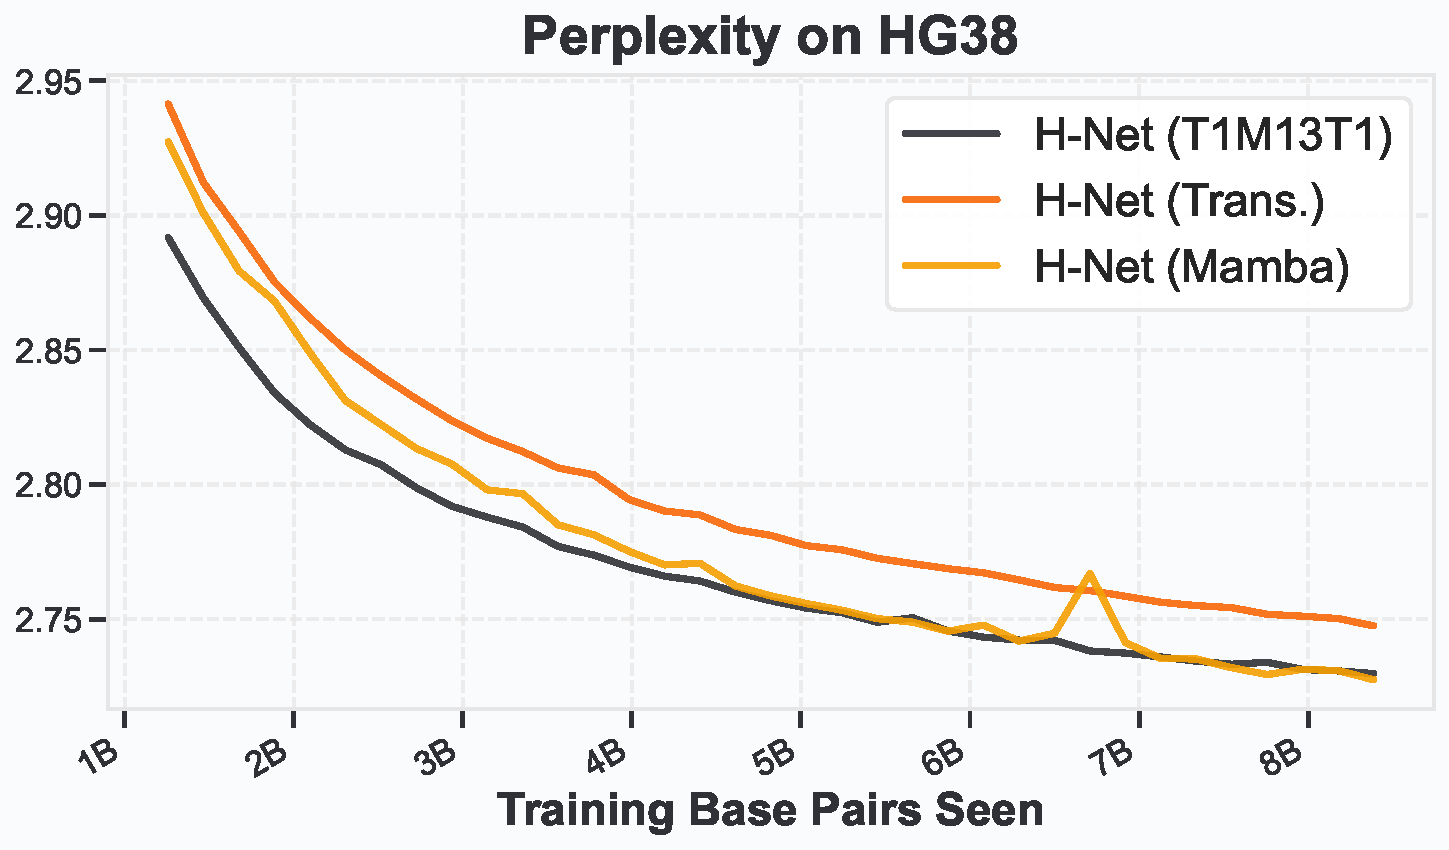
\includegraphics[width=\linewidth]{fig_img/dna_m4.pdf} 
            \captionof{figure}{
            \textbf{Mamba-2-only encoder loss curves} during the stable phase of training.
            The pure Mamba-2 model is more unstable with a loss spike. Adding Transformer layers to the \main{} near the DC modules can alleviate instabilities.
            \model{} (1-stage, principled) corresponds to the \colorbox{Main}{T1M13T1} \main{} architecture.
            }
            \label{fig: dna_supp}
        \end{minipage}
    \end{minipage}
\end{figure}

